Slope fields are useful for two things: \textbf{reading behavior quickly} and \textbf{sketching solutions when algebra is hard}.

\subsubsection*{Read a slope field (fast workflow)}
\begin{enumerate}[leftmargin=*]
  \item \textbf{Mark zero-slope curves:} solve $f(x,y)=0$ in $y'=f(x,y)$. These are horizontal tangent locations.
  \item \textbf{Check sign regions:} where $f(x,y)>0$, solutions rise; where $f(x,y)<0$, solutions fall.
  \item \textbf{Estimate speed of change:} larger $|f(x,y)|$ means steeper segments and faster change.
  \item \textbf{Use the initial condition:} the particular solution must pass through the given point and follow local segment directions.
\end{enumerate}

\subsubsection*{Draw a slope field (quick method)}
For $y'=f(x,y)$:
\begin{enumerate}[leftmargin=*]
  \item Choose a rectangular grid of points.
  \item At each grid point $(x_i,y_j)$, compute $m_{ij}=f(x_i,y_j)$.
  \item Draw a short line segment with slope $m_{ij}$ (keep segment lengths similar).
  \item Add key guide curves first (for example, $f(x,y)=0$ and any undefined lines).
  \item Sketch solution curves as smooth paths tangent to the local segments.
\end{enumerate}

\subsubsection*{Three compact visual examples}
\begin{center}
\begin{minipage}[t]{0.32\textwidth}
\centering
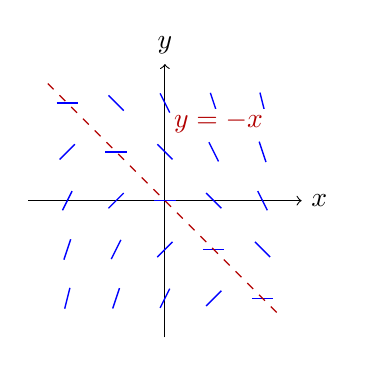
\begin{tikzpicture}[scale=0.62]
  \draw[->] (-2.8,0) -- (2.8,0) node[right] {$x$};
  \draw[->] (0,-2.8) -- (0,2.8) node[above] {$y$};
  \foreach \X in {-2,-1,0,1,2} {
    \foreach \Y in {-2,-1,0,1,2} {
      \pgfmathsetmacro{\M}{-(\X)-(\Y)}
      \pgfmathsetmacro{\A}{atan(\M)}
      \draw[blue, line width=0.5pt]
        ({\X-0.22*cos(\A)},{\Y-0.22*sin(\A)})
        --
        ({\X+0.22*cos(\A)},{\Y+0.22*sin(\A)});
    }
  }
  \draw[dashed, red!70!black] (-2.4,2.4) -- (2.4,-2.4);
  \node[red!70!black, fill=white, inner sep=1pt] at (1.1,1.6) {$y=-x$};
\end{tikzpicture}

\small \textbf{Example 1:} $y'=-x-y$
\end{minipage}\hfill
\begin{minipage}[t]{0.32\textwidth}
\centering
\begin{tikzpicture}[scale=0.62]
  \draw[->] (-2.8,0) -- (2.8,0) node[right] {$x$};
  \draw[->] (0,-2.8) -- (0,2.8) node[above] {$y$};
  \foreach \X in {-2,-1,0,1,2} {
    \foreach \Y in {-2,-1,0,1,2} {
      \pgfmathsetmacro{\M}{(\X)*(\Y)}
      \pgfmathsetmacro{\A}{atan(\M)}
      \draw[blue, line width=0.5pt]
        ({\X-0.22*cos(\A)},{\Y-0.22*sin(\A)})
        --
        ({\X+0.22*cos(\A)},{\Y+0.22*sin(\A)});
    }
  }
  \draw[dashed, red!70!black] (0,-2.5) -- (0,2.5);
  \draw[dashed, red!70!black] (-2.5,0) -- (2.5,0);
  \node[red!70!black, fill=white, inner sep=1pt] at (1.45,0.45) {$y=0$};
  \node[red!70!black, fill=white, inner sep=1pt, rotate=90] at (0.42,1.55) {$x=0$};
\end{tikzpicture}

\small \textbf{Example 2:} $y'=xy$
\end{minipage}\hfill
\begin{minipage}[t]{0.32\textwidth}
\centering
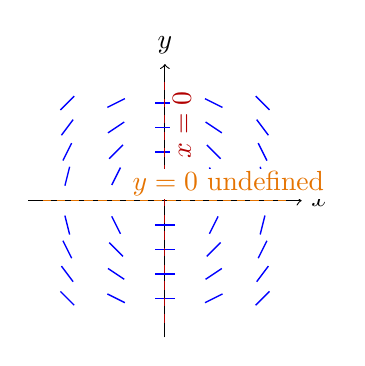
\begin{tikzpicture}[scale=0.62]
  \draw[->] (-2.8,0) -- (2.8,0) node[right] {$x$};
  \draw[->] (0,-2.8) -- (0,2.8) node[above] {$y$};
  \foreach \X in {-2,-1,0,1,2} {
    \foreach \Y in {-2,-1.5,-1,-0.5,0.5,1,1.5,2} {
      \pgfmathsetmacro{\M}{-(\X)/(\Y)}
      \pgfmathsetmacro{\A}{atan(\M)}
      \draw[blue, line width=0.5pt]
        ({\X-0.2*cos(\A)},{\Y-0.2*sin(\A)})
        --
        ({\X+0.2*cos(\A)},{\Y+0.2*sin(\A)});
    }
  }
  \draw[dashed, red!70!black] (0,-2.5) -- (0,2.5);
  \draw[densely dashed, orange!90!black] (-2.5,0) -- (2.5,0);
  \node[red!70!black, fill=white, inner sep=1pt, rotate=90] at (0.35,1.55) {$x=0$};
  \node[orange!90!black, fill=white, inner sep=1pt] at (1.3,0.35) {$y=0$ undefined};
\end{tikzpicture}

\small \textbf{Example 3:} $yy'+x=0$
\end{minipage}
\end{center}

\begin{itemize}[leftmargin=*]
  \item \textbf{Example 1:} $y=-x$ is the zero-slope isocline. Above it slopes are negative; below it slopes are positive.
  \item \textbf{Example 2:} the axes are zero-slope guide lines because $xy=0$ whenever $x=0$ or $y=0$.
  \item \textbf{Example 3:} rewriting as $y'=-\dfrac{x}{y}$ shows a zero-slope isocline at $x=0$ and an undefined line at $y=0$.
\end{itemize}

\subsubsection*{Common mistakes}
\begin{itemize}[leftmargin=*]
  \item Drawing curves that cut across local segment directions.
  \item Treating slope marks as disconnected graph pieces rather than tangent information.
  \item Giving only a sketch when the question also asks for long-run behavior in words.
\end{itemize}
